% --------------------------------------
% Document Class
% --------------------------------------
\documentclass[11pt]{article}
% --------------------------------------



% --------------------------------------
% Use Package
% --------------------------------------

% french, english
\usepackage[francais]{babel}

% font, french accent
\usepackage[utf8]{inputenc} 
\usepackage[T1]{fontenc} 

% page layout
\usepackage{geometry}

% hypertext link
\usepackage[pdfpagelabels]{hyperref}

\usepackage{graphicx}
\usepackage{float}
\usepackage{verbatim}
\usepackage{fancyhdr}
\usepackage{amsmath}


% include pdf
\usepackage[final]{pdfpages}

% insert code
\usepackage{listings}

% define our color
\usepackage{xcolor}

% code color
\definecolor{ligthyellow}{RGB}{250,247,220}
\definecolor{darkblue}{RGB}{5,10,85}
\definecolor{ligthblue}{RGB}{1,147,128}
\definecolor{darkgreen}{RGB}{8,120,51}
\definecolor{darkred}{RGB}{160,0,0}

% other color
\definecolor{ivi}{RGB}{141,107,185}


\lstset{
    language=R,
    captionpos=b,
    extendedchars=true,
    frame=lines,
    numbers=left,
    numberstyle=\tiny,
    numbersep=5pt,
    keepspaces=true,
    breaklines=true,
    showspaces=false,
    showstringspaces=false,
    breakatwhitespace=false,
    stepnumber=1,
    showtabs=false,
    tabsize=3,
    basicstyle=\small\ttfamily,
    backgroundcolor=\color{ligthyellow},
    keywordstyle=\color{ligthblue},
    morekeywords={include, printf, uchar},
    identifierstyle=\color{darkblue},
    commentstyle=\color{darkgreen},
    stringstyle=\color{darkred},
}


% --------------------------------------



% --------------------------------------
% Page setting
% --------------------------------------
%\pagestyle{empty}
\setlength{\headheight}{15pt}

\setcounter{secnumdepth}{3}
\setcounter{tocdepth}{2}

\makeatletter
\@addtoreset{chapter}{part}
\makeatother 

\hypersetup{         % parametrage des hyperliens
  colorlinks=true,      % colorise les liens
  breaklinks=true,      % permet les retours à la ligne pour les liens trop longs
  urlcolor= blue,       % couleur des hyperliens
  linkcolor= black,     % couleur des liens internes aux documents (index, figures, tableaux, equations,...)
  citecolor= green      % couleur des liens vers les references bibliographiques
}

% --------------------------------------

% --------------------------------------
% Information
% --------------------------------------
\title{Compte-rendu TP3 RdF : Segmentation par binarisation}
\author{Elliot VANEGUE et Gaëtan DEFLANDRE}
% --------------------------------------



% --------------------------------------
% Begin content
% --------------------------------------
\begin{document}

  % Set language to english
  \selectlanguage{francais}

  % Start the page counting
  \pagenumbering{arabic}

  \maketitle
  
  \mbox{}
  \newpage
  \clearpage
  
  \section*{Introduction}
  Lors de ce TP, nous allons aborder différentes manières de segmenter une image par 
  classification de ses pixels. Le but de la segmentation est de  conserver les pixels d'un 
  objet et ignorer les pixels du fond. Nous mettrons en avant, plusieurs méthodes permettant 
  de déterminer un seuil de binarisation. Nous verrons ainsi leurs avantages et inconvénients.\\
  
  D'abord, nous chercherons le meilleur seuil à partir de l'histogramme de niveaux de gris.
  Ensuite, nous fixerons ce seuil à l'aide de l'histogramme de niveaux de texture.
  Enfin, nous combinerons les deux techniques afin d'obtenir une méthode encore plus 
  fiable pour la segmentation.\\
  
  
  
  \section{Histogramme des niveaux de gris}
  
  Dans le but conserver uniquement pixels des disques, pour les images d'exemples. Nous allons segmenter ces
  images avec la techniques du seuillages. Seuiller ou binariser une image consiste conserver les pixels dont
  la valeur est au-dessus d'un seuil et rejeter les pixels de valeurs infèrieurs ou égales à ce seuil.\\
  
  \begin{figure}[H]
    \center
    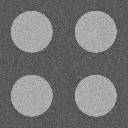
\includegraphics[width=2.5cm]{texture-0/texture-0.png}
    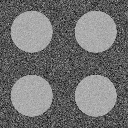
\includegraphics[width=2.5cm]{texture-1/texture-1.png}
    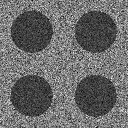
\includegraphics[width=2.5cm]{texture-2/texture-2.png}
    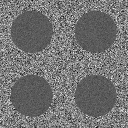
\includegraphics[width=2.5cm]{texture-3/texture-3.png}
    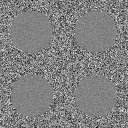
\includegraphics[width=2.5cm]{texture-4/texture-4.png}
    \caption{Les images utilisées pour les testes}
  \end{figure}
  
  Pour déterminer la valeur du seuil, nous allons nous intéresser à l'histogramme des niveaux de gris. Pour 
  afficher l'histogramme en langage R, nous utilisons la fonction \textit{hist} des bibliothèques du langage.
  En R, l'intensité des pixels varis de 0 à 1 et une image 8 bits est consistitué de 256 niveaux de gris.
  Il faut alors donne en paramètre à l'histogramme tous les niveaux. C'est la fonction \textit{seq} qui
  découpe l'intervalle [0;1] en \textit{nbins}, avec \textit{nbins} le nombre de niveaux de gris (256).\\
  
  \newpage
  
  Voici les lignes permettant d'afficher l'histogramme d'une image :
  
  \begin{lstlisting}[caption=Afficher l'histogramme d'une image]
# Chargement d'une image
nom <- "rdf-2-classes-texture-0.png"
image <- rdfReadGreyImage (nom)

# Calcul et affichage de l'histogramme
nbins <- 256
h <- hist (as.vector (image), breaks = seq (0, 1, 1 / nbins))\end{lstlisting}

  Une fois l'histogramme afficher, nous remarquons que, pour les premières textures, deux pics apparaisent. 
  Ils conrespondent aux niveaux de gris des disques et aux niveaux de gris du fond. Nous prennons une valeur 
  entre ces deux pics comme seuil, pour binariser nos images.
  
  \begin{figure}[H]
    \center
    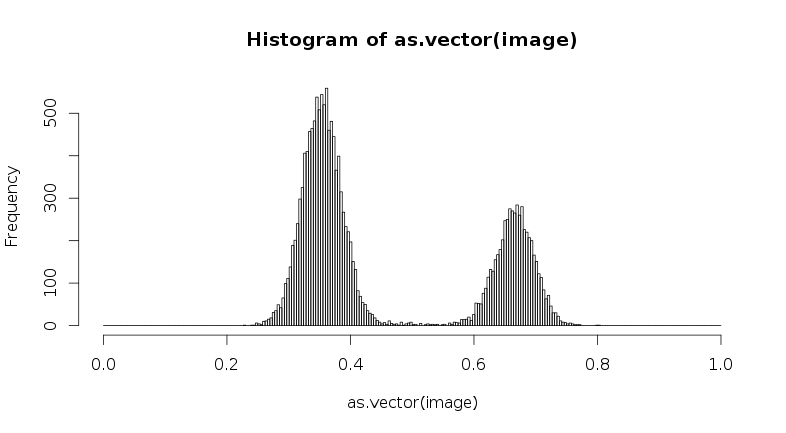
\includegraphics[width=14cm]{../elliot/gris0.png}
    \caption{Histogramme des gris de la texture 0}
  \end{figure}

  
   \begin{center}
    \begin{tabular}{|c|c|c|c|}
      \hline
      \textbf{Image source} & \textbf{Histogramme des gris} & \textbf{Image binarisée} & \textbf{Taux erreurs (\%)}\\
      \hline
      \shortstack{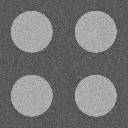
\includegraphics[width=3cm]{texture-0/texture-0.png} \\ \tiny{rdf-2-classes-texture-0.png}} & 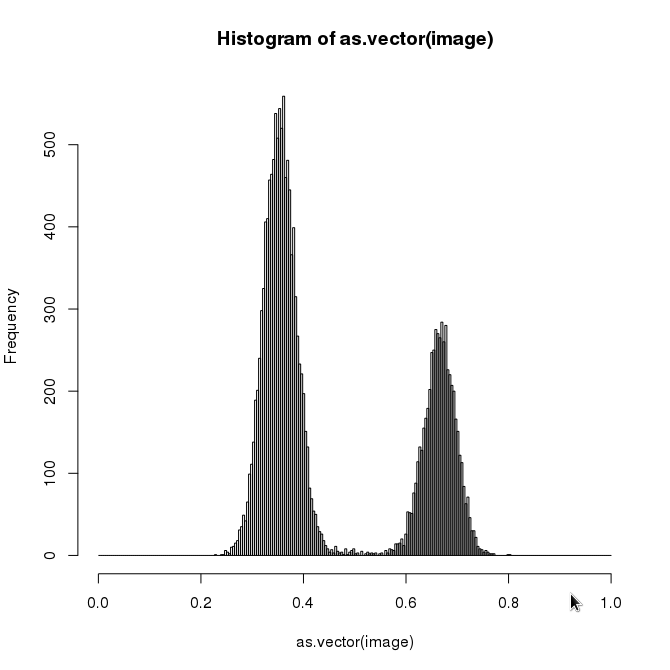
\includegraphics[width=4cm]{texture-0/texture-0-1-hist.png} & \shortstack{
\includegraphics[width=3cm]{texture-0/texture-0-2-bin-gris.png} \\ \small{Seuil : 0,5}  } & 0.1159668\\
      \hline
      \shortstack{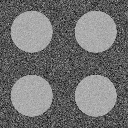
\includegraphics[width=3cm]{texture-1/texture-1.png} \\ \tiny{rdf-2-classes-texture-1.png}} & 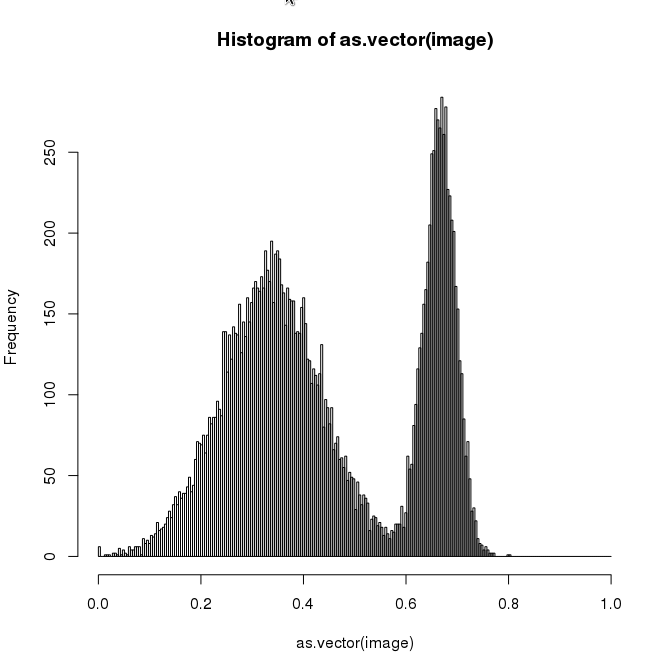
\includegraphics[width=4cm]{texture-1/texture-1-1-hist.png} & \shortstack{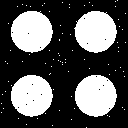
\includegraphics[width=3cm]{texture-1/texture-1-2-bin-gris.png} \\ \small{Seuil : 0,58} } & 0.8850098\\
      \hline
      \shortstack{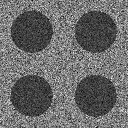
\includegraphics[width=3cm]{texture-2/texture-2.png} \\ \tiny{rdf-2-classes-texture-2.png}} & 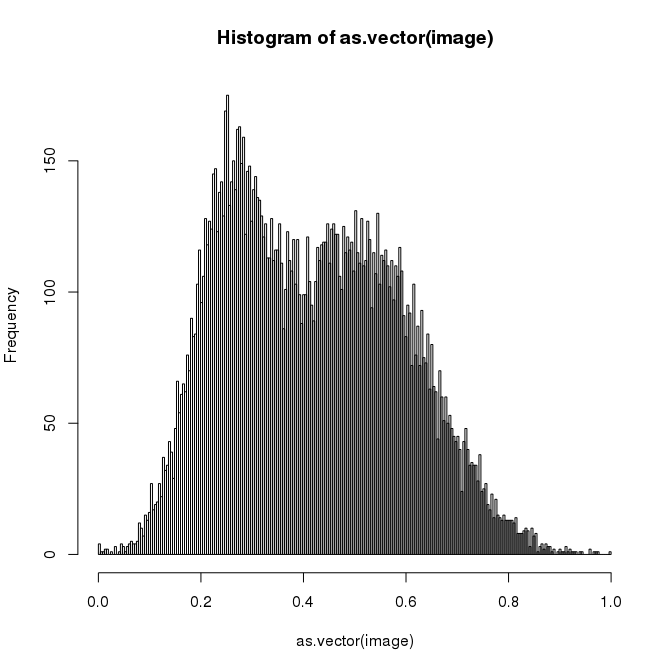
\includegraphics[width=4cm]{texture-2/texture-2-1-hist.png} & \shortstack{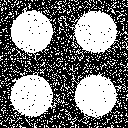
\includegraphics[width=3cm]{texture-2/texture-2-2-bin-gris.png} \\ \small{Seuil : 0,39} } & 15.58838\\
      \hline
      \shortstack{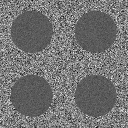
\includegraphics[width=3cm]{texture-3/texture-3.png} \\ \tiny{rdf-2-classes-texture-3.png}} & 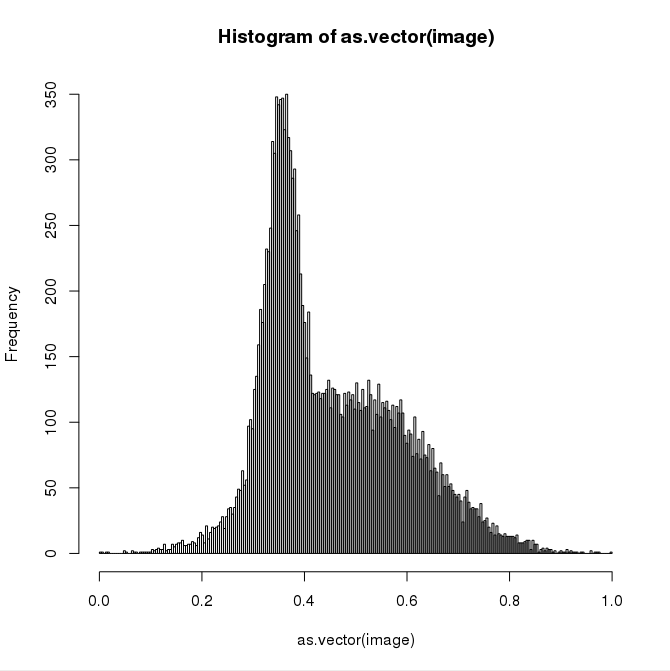
\includegraphics[width=4cm]{texture-3/texture-3-1-hist.png} & \shortstack{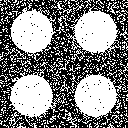
\includegraphics[width=3cm]{texture-3/texture-3-2-bin-gris.png} \\ \small{Seuil : 0,42} } & 19.6167\\
      \hline
      \shortstack{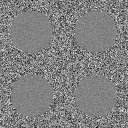
\includegraphics[width=3cm]{texture-4/texture-4.png} \\ \tiny{rdf-2-classes-texture-4.png}} & 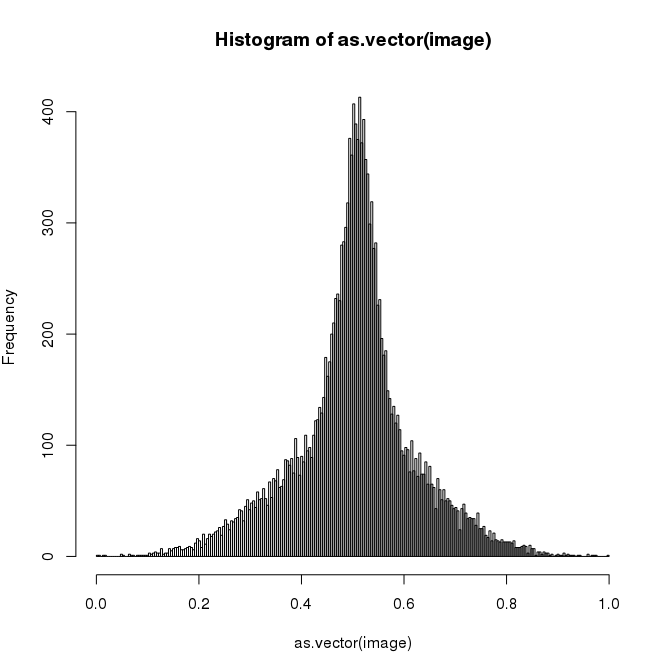
\includegraphics[width=4cm]{texture-4/texture-4-1-hist.png} & \shortstack{
\includegraphics[width=3cm]{texture-4/texture-4-2-bin-gris.png} \\ \small{Seuil : 0,5}  } & 45.89233\\
      \hline
    \end{tabular}
  \end{center}
  
  \subsection*{Conclusion sur les résultats de l'histogramme de niveaux de gris}
  
  Lorsque les images sont de bonne qualité (texture 0 et 1) ont retrouve facilement sur l'histogramme, les deux 
  pics précedemment cités et un creux entre les deux. Celà nous permettant d'obtenir un seuil assez fiable.\\

  Cependant quand les images à binariser sont trop détériorer (texutre 2 et 3), avec beaucoup de bruit. 
  L'histogramme des niveaux de gris, ne nous permet pas de déterminer un seuil précisément. \\

  Pour la texture 4, en plus d'être fortement bruitée, les niveaux de gris de l'image sont proches. Il est 
  impossible de déterminer un seuil uniquement avec son histogramme.\\
  
  \section{Histogramme des niveaux de texture}
  
  Une autre alternative, pour la classification des pixels est de déterminer le seuil à l'aide de 
  l'histogramme des niveaux de texture. Pour trouver cette histogramme il faut calculer l'écart-type,
  obtenu grâce à la fonction \textit{rdfTextureEcartType}, diffèrent de écart-type de l'image, car ici 
  c'est la diffèrence entre l'image et l'image moyenné qui est utilisée. L'image moyenné est obtenu avec 
  la fonction \textit{rdfMoyenneImage}.\\
  
  \begin{figure}[H]
    \center
    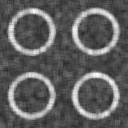
\includegraphics[width=4cm]{texture-0/texture-0-5-ecart-type.png}
    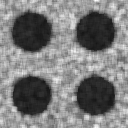
\includegraphics[width=4cm]{texture-4/texture-4-5-ecart-type.png}
    \caption{A gauche, écart-type de la texture 0. A droite, écart-type de la texture 4.}
  \end{figure}
  
  La moyenne de l'image effectué sur un voisinnage. La dimension de la matrice de voisin peut être contrôler 
  grace au paramètre \textit{taille} passé aux fonctions. Ce paramètre, tel un rayon, indique le nombre de 
  pixels à prendre en compte autour du pixel cible. Si le taille = 2 alors masque sera une matrice de 5*5 
  pixels.\\
  
  \newpage
  
  Ci-dessous les lignes permettant d'afficher l'histogramme de niveaux de texture d'une image :
  \begin{lstlisting}[caption=Afficher l'histogramme de niveaux de texture d'une image]
# Chargement d'une image
nom <- "rdf-2-classes-texture-3.png"
image <- rdfReadGreyImage (nom)

o <- rdfTextureEcartType(image, 2)

# Calcul et affichage de son histogramme
nbins <- 256
h <- hist (as.vector (o), breaks = seq (0, 1, 1 / nbins))\end{lstlisting}
  
  \begin{figure}[H]
    \center
    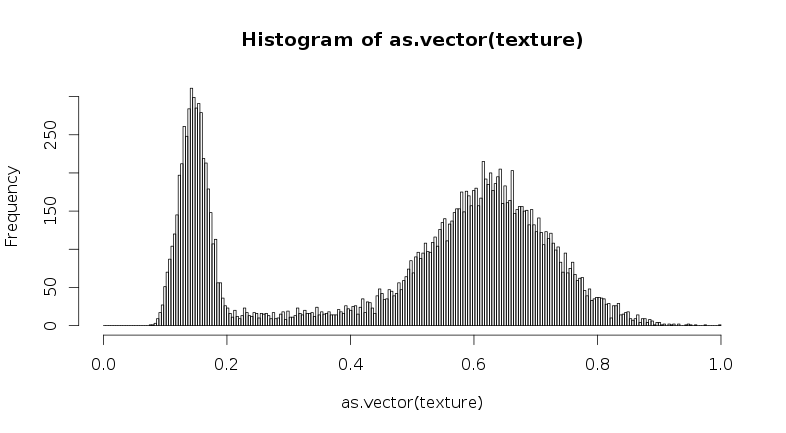
\includegraphics[width=14cm]{../elliot/texture4.png}
    \caption{Histogramme de texture de la texture 4.}
  \end{figure}
  
     \begin{center}
    \begin{tabular}{|c|c|c|c|}
      \hline
      \textbf{Image source} & \textbf{Histogramme de texture} & \textbf{Image binarisée} & \textbf{Taux erreurs (\%)}\\
      \hline
      \shortstack{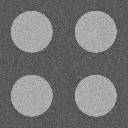
\includegraphics[width=3cm]{texture-0/texture-0.png} \\ \tiny{rdf-2-classes-texture-0.png}} & 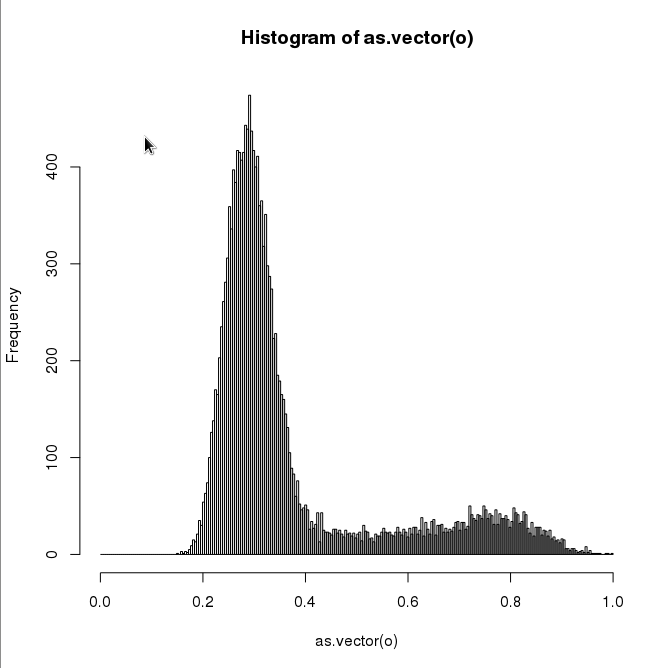
\includegraphics[width=4cm]{texture-0/texture-0-3-hist-ecart-type.png} & \shortstack{
\includegraphics[width=3cm]{texture-0/texture-0-4-bin-tex.png} \\ \small{Seuil : 0,5}  } & 0.1159668\\
      \hline
      \shortstack{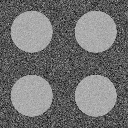
\includegraphics[width=3cm]{texture-1/texture-1.png} \\ \tiny{rdf-2-classes-texture-1.png}} & 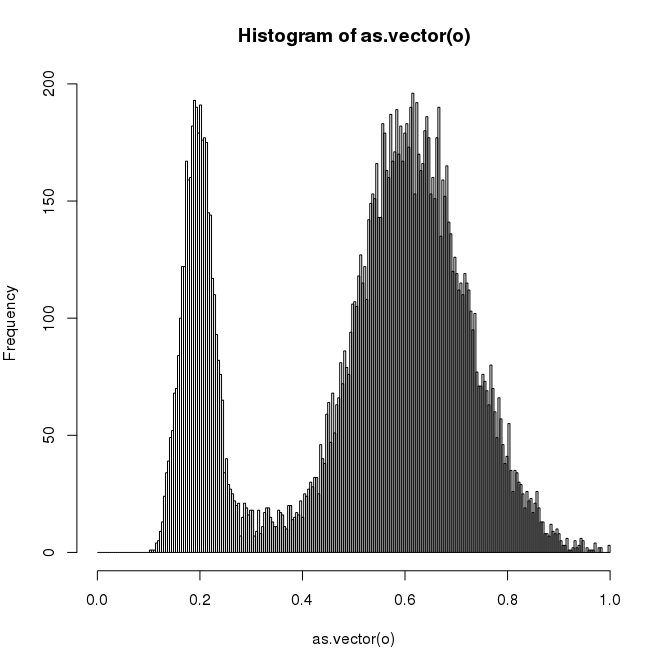
\includegraphics[width=4cm]{texture-1/texture-1-3-hist-ecart-type.png} & \shortstack{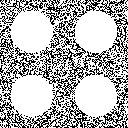
\includegraphics[width=3cm]{texture-1/texture-1-4-bin-tex.png} \\ \small{Seuil : 0,32} } & 37.42065\\
      \hline
      \shortstack{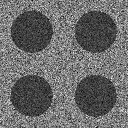
\includegraphics[width=3cm]{texture-2/texture-2.png} \\ \tiny{rdf-2-classes-texture-2.png}} & 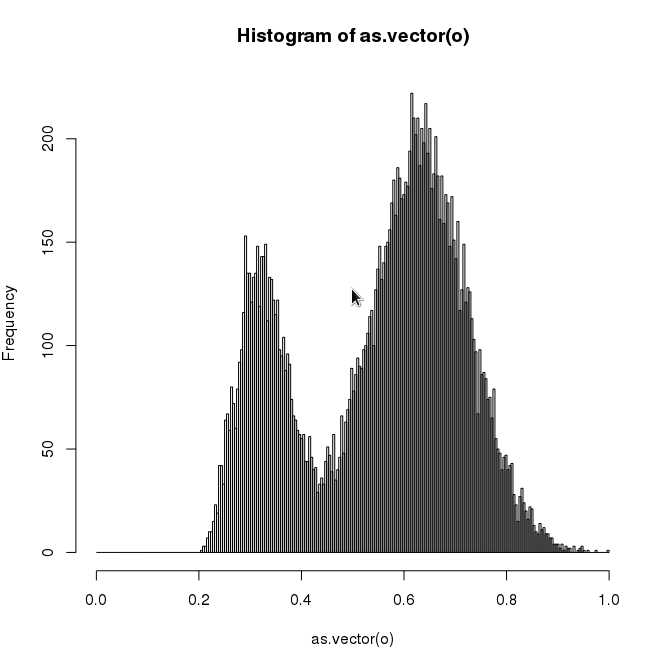
\includegraphics[width=4cm]{texture-2/texture-2-3-hist-ecart-type.png} & \shortstack{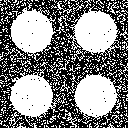
\includegraphics[width=3cm]{texture-2/texture-2-4-bin-tex.png} \\ \small{Seuil : 0,42} } & 19.49463\\
      \hline
      \shortstack{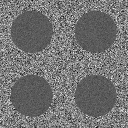
\includegraphics[width=3cm]{texture-3/texture-3.png} \\ \tiny{rdf-2-classes-texture-3.png}} & 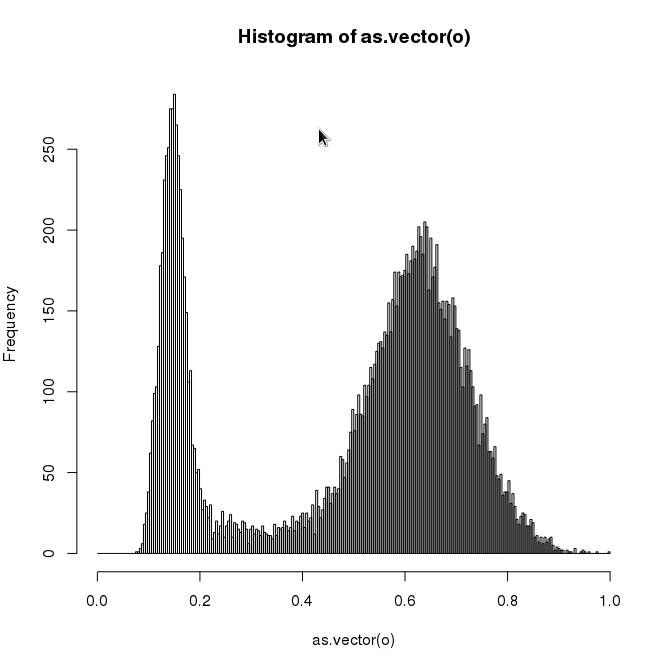
\includegraphics[width=4cm]{texture-3/texture-3-3-hist-ecart-type.png} & \shortstack{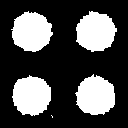
\includegraphics[width=3cm]{texture-3/texture-3-4-bin-tex.png} \\ \small{Seuil : 0,36} } & 25.28076\\
      \hline
      \shortstack{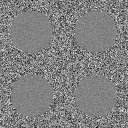
\includegraphics[width=3cm]{texture-4/texture-4.png} \\ \tiny{rdf-2-classes-texture-4.png}} & 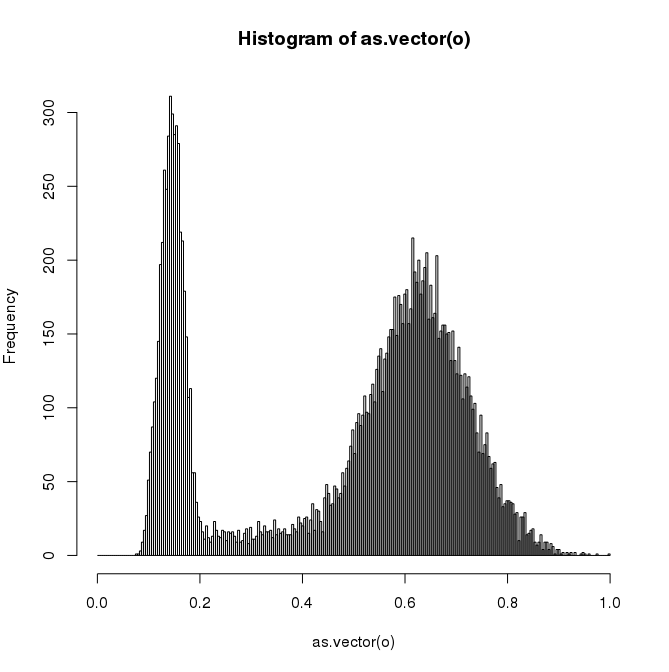
\includegraphics[width=4cm]{texture-4/texture-4-3-hist-ecart-type.png} & \shortstack{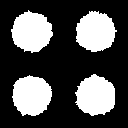
\includegraphics[width=3cm]{texture-4/texture-4-4-bin-tex.png} \\ \small{Seuil : 0,35}  } & 56.70776\\
      \hline
    \end{tabular}
  \end{center}
  
  \subsection*{Conclusion sur les résultats de l'histogramme de niveaux de texture}
  Il est plus facile de déterminer un seuil avec l'histoigramme de texture, pour les images qui sont 
  plus détérioré par le bruit. Néanmoins, le taux d'erreur n'est pas forcement plus faible. Nous 
  pouvons noter que, pour la texture 4, même si son taux d'erreurs est plus élevé avec cette technique 
  les disques sont mieux segmenter. Tous les pixels des disques de premier plan sont reconnu, or le 
  fond n'est pas correctement ignoré. Ceci est directement lié à la technique du seuillage et aux ton 
  de gris  très proches entre les pixels des disques et ceux du fond. On ne peut que difficilement 
  faire mieux avec un seuillage.\\
  
  Par conséquent, la méthodes de ségmentation avec l'histogramme des textures, permet de retrouver 
  un seuil pour segmenter une image quand l'histogramme de gris ne le permet pas, mais les résultat 
  ne sont pas fiable dans tous les cas.\\
  
  \section{Histogramme conjoint}
  
       \begin{center}
    \begin{tabular}{|c|c|c|c|}
      \hline
      \textbf{Image source} & \textbf{Image écart-type} & \textbf{Histogramme 2D} & \textbf{Taux erreurs (\%)}\\
      \hline
      \shortstack{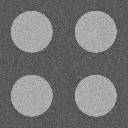
\includegraphics[width=3cm]{texture-0/texture-0.png} \\ \tiny{rdf-2-classes-texture-0.png}} & 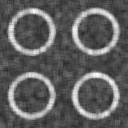
\includegraphics[width=3cm]{texture-0/texture-0-5-ecart-type.png} & 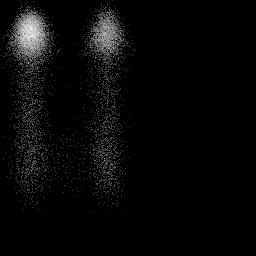
\includegraphics[width=3cm]{texture-0/texture-0-6-h2d.png} & ?\\
      \hline
      \shortstack{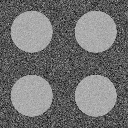
\includegraphics[width=3cm]{texture-1/texture-1.png} \\ \tiny{rdf-2-classes-texture-1.png}} & 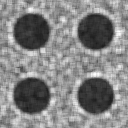
\includegraphics[width=3cm]{texture-1/texture-1-5-ecart-type.png} & 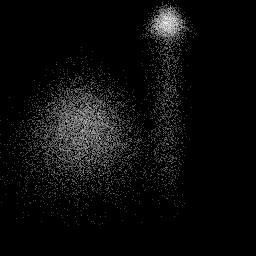
\includegraphics[width=3cm]{texture-1/texture-1-6-h2d.png} & ?\\
      \hline
      \shortstack{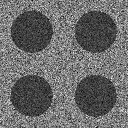
\includegraphics[width=3cm]{texture-2/texture-2.png} \\ \tiny{rdf-2-classes-texture-2.png}} & 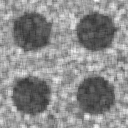
\includegraphics[width=3cm]{texture-2/texture-2-5-ecart-type.png} & 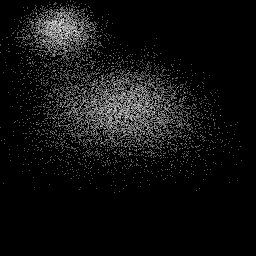
\includegraphics[width=3cm]{texture-2/texture-2-6-h2d.png} & ?\\
      \hline
      \shortstack{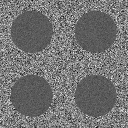
\includegraphics[width=3cm]{texture-3/texture-3.png} \\ \tiny{rdf-2-classes-texture-3.png}} & 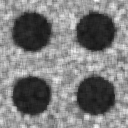
\includegraphics[width=3cm]{texture-3/texture-3-5-ecart-type.png} & \includegraphics[width=3cm]{texture-3/texture-3-6-h2d.png} & ?\\
      \hline
      \shortstack{\includegraphics[width=3cm]{texture-4/texture-4.png} \\ \tiny{rdf-2-classes-texture-4.png}} & \includegraphics[width=3cm]{texture-4/texture-4-5-ecart-type.png} & \includegraphics[width=3cm]{texture-4/texture-4-6-h2d.png} & ?\\
      \hline
    \end{tabular}
  \end{center}
    
  \section*{Conclusion}


\end{document}
